% EPC flow charts
% Author: Fabian Schuh
\documentclass{article}
\usepackage[inner=0.5in,outer=0.5in,top=0.25in,bottom=0.25in]{geometry}
\usepackage{xeCJK} % 分開設置中英文字型
\setCJKmainfont{微軟正黑體} % 設定中文字型
\usepackage{enumitem}
\usepackage{graphicx}
\usepackage{tikz}
\usetikzlibrary{positioning,arrows}
\usetikzlibrary{shapes.multipart}

\tikzset{
    state/.style={
           rectangle,
           rounded corners,
           draw=black,
           minimum height=2em,
           inner sep=2pt,
           text centered,
           },
}
\tikzset{
    phantom/.style={
           rectangle,
           rounded corners,
           minimum height=2em,
           inner sep=2pt,
           text centered,
           },
}
\setlist[enumerate]{topsep = 0pt, noitemsep}%remove extra empty spaces above enumerate envr, and make the items more compact

\begin{document}
\tikzstyle{abstract}=[rectangle, draw=black, rounded corners,  anchor=center, text width=3cm,text centered,rectangle split, rectangle split parts=2]

\begin{tikzpicture}[item/.style={draw=black, rounded corners,  anchor=center, text width=8.5cm,align = center,rectangle split, rectangle split parts=#1, rectangle split part align={center, left} }]

\begin{scope}[node distance=5mm and 5mm]

\node [ item=4](a) at (1,1) {%
            \textbf{weekly routine}
            \nodepart{two}
            \begin{enumerate}
            	\item thinkpad T60 電池找
            	\item SMEG烤箱時間溫度表製作
            	\item compressor 排水閥, still no clue, dangerous
           \end{enumerate}
           \nodepart{three}\textbf{特色}
	\nodepart{four}
            \begin{enumerate}
            	\item 使用LYX與SW,高度自動化產生django-compatible html(省下很多細微瑣碎步驟)。
            	\item 讓SW與LYX產生的網頁能夠正確顯示。如SW export links時有點問題,要記錄下可行步驟,並嘗試自動化。
           \end{enumerate}
            };

\node [phantom, inner sep = 0pt, right=of a.north east](center_point){};

\node [above = of center_point, align = center] (title){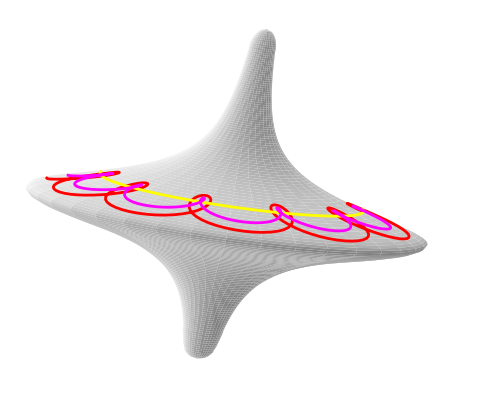
\includegraphics[width=0.4\textwidth]{../../figs/logo_June27_2016.png}\\ \LARGE fixing \& crafting};

\node [state,below=of a](b)
{git log}edge [<-,>=stealth'] (a);

\node [ item=2, right = of center_point, anchor = north west](small) {%
            \textbf{weekly routine}
            \nodepart{two}
            \begin{enumerate}
            	\item 查怎麼修
           \end{enumerate}
            };

\end{scope}
\end{tikzpicture}
\end{document}